\section{Experimental results}
\label{sec:experimental_results}
The proposed hardware/software framework is demonstrated on a Xilinx Zynq-7020 SoC (Zybo-Z7 development board). We deploy TFLite micro on the processing system (PS), and we implement the proposed hardware architecture on the programmable logic (PL). We address a design exploration by building and training custom CNN models in TF, and evaluating their computational and accuracy performance on the proposed hardware architecture.

build and train two CNN-based models for CIFAR-10 dataset classification

The PS ARM Cortex-A9 CPU at 666MHz, this processor includes NEON SIMD Engine and single/double precision floating-point unit (FPU)\cite{xilinx2015zynq}.

In this platform, we implement the proposed hardware/software solution to deploy TFLite models on the Zynq-7020 network structure shown in \fig{fig:sbs_network} for handwritten digit classification task using MNIST data set. The SbS model is trained in Matlab without any quantization method, using standard floating-point. The resulting synaptic weight matrices are deployed on the embedded system. There, the SbS network is built as a sequential model using the API from the SbS embedded software framework \cite{nevarez2020accelerator}. This API allows to configure the computational workload of the neural network, which can be distributed among the hardware processing units and the embedded CPU.

For the evaluation of our approach, we address a design exploration by reviewing the computational latency, inference accuracy, resource utilization, and power dissipation. First, we benchmark the performance of SbS network simulation on the embedded CPU, and then repeat the measurements on hardware processing units with standard floating-point computation. Afterwards, we evaluate our dot-product architecture, addressing a design exploration with hybrid custom floating-point approximation, as well as the hybrid logarithmic approximation. Finally, we present a discussion of the presented results.

\subsection{Computational performance}
\subsubsection{Conv2D operator}
\subsubsection{DepthwiseConv2D operator}
\subsection{Accuracy performance}


\begin{figure}[t!]
	\centering
	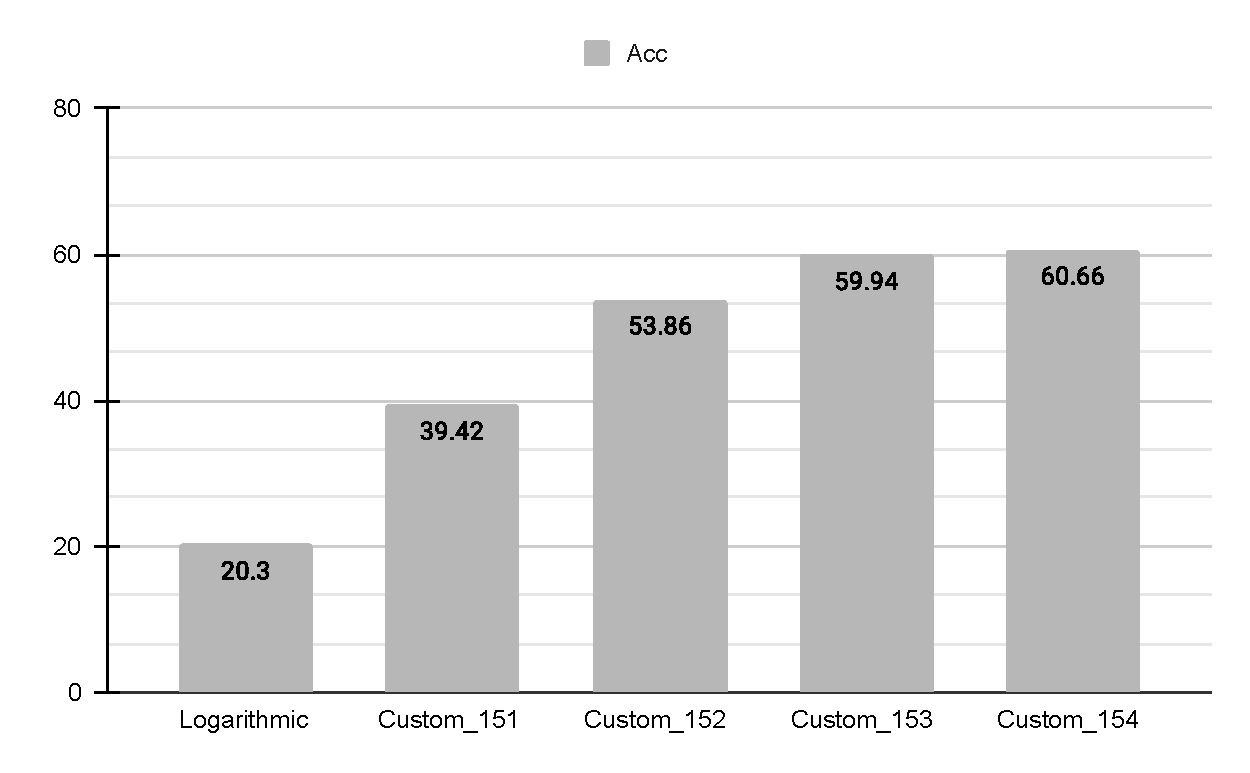
\includegraphics[width=0.5\textwidth]{../figures/acc_depthwise_cifar_custom.pdf}
	\caption{Accuracy performance of depthwise separable CNN architecture with custom floating-point approximation.}
	\label{fig:acc_custom}
\end{figure}

\begin{figure}[t!]
	\centering
	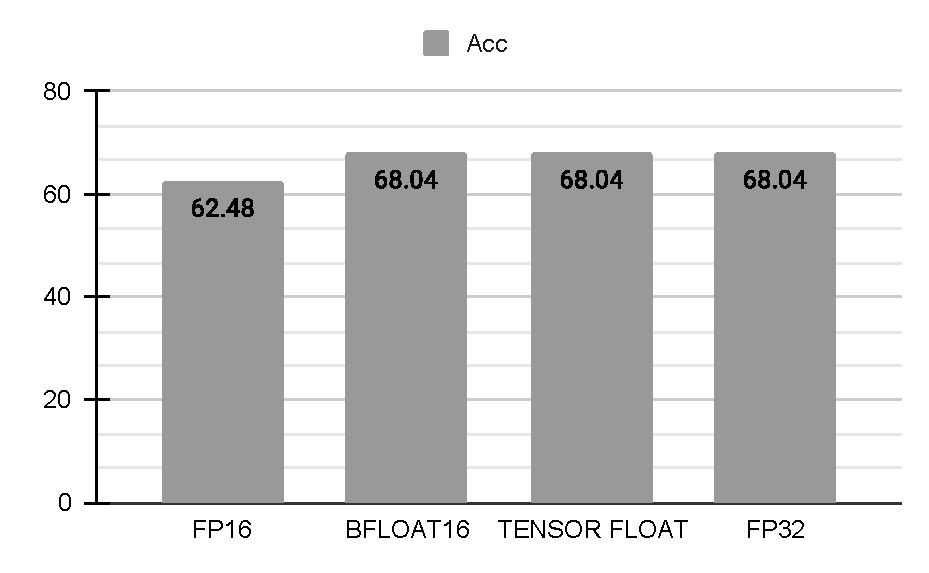
\includegraphics[width=0.5\textwidth]{../figures/acc_depthwise_cifar_standard.pdf}
	\caption{Accuracy performance of depthwise separable CNN architecture with standard floating-point formats.}
	\label{fig:acc_standard}
\end{figure}